\documentclass[12pt]{article}

\usepackage{bbm}
\usepackage{fancyhdr}
\usepackage{titling}
\usepackage{enumitem}
\usepackage{amsmath}
\usepackage{dsfont}
\usepackage{amsfonts}
\usepackage{amssymb}
\usepackage{amsthm}
\usepackage{geometry}
\usepackage{tikz}
\usepackage{algorithm}
\usepackage{algpseudocode}
\geometry{verbose,tmargin=1in,bmargin=1in,lmargin=1in,rmargin=1in}
\renewcommand{\vec}[1]{\mathbf{#1}}
\newcommand{\dec}{\text{dec}}
\newcommand{\divi}{\mathbin{\textnormal{div}}}
\title{Homework 1}
\author{Satvik Prasad}
\date{}
\newtheorem{lemma}{Lemma}[section]
\fancypagestyle{plain}{%
  \fancyhf{}
  \fancyhead[L]{\theauthor}
  \fancyhead[R]{\thedate}
}
\pagestyle{plain}
\makeatletter
\def\@maketitle{%
  \newpage
  \null
  \vskip 1em%
  \begin{center}%
    \let \footnote \thanks
    {\LARGE \@title \par}%
    \vskip 1em%
  \end{center}%
  \par
\vskip 1em}
\makeatother
\usepackage{cmbright}

\newcommand{\mat}[1]{\mathbf{#1}}

% ---------- Probability theory ----------
% Core operators (optional argument-free; use as \E{X}, \Var{X}, \Cov{X}{Y})
\DeclareMathOperator{\EOp}{\mathbb{E}}
\DeclareMathOperator{\VarOp}{Var}
\DeclareMathOperator{\CovOp}{Cov}
\DeclareMathOperator{\CorrOp}{Corr}

\renewcommand{\P}[1]{\mathbb{P}\left(#1\right)}        % \P{A}
\newcommand{\E}[1]{\EOp\left[#1\right]}                % \E{X}
\newcommand{\Var}[1]{\VarOp\left(#1\right)}            % \Var{X}
\newcommand{\Cov}[2]{\CovOp\left(#1,\,#2\right)}       % \Cov{X}{Y}
\newcommand{\Corr}[2]{\CorrOp\left(#1,\,#2\right)}     % \Corr{X}{Y}
\newcommand{\SD}[1]{\operatorname{SD}\left(#1\right)}  % \SD{X}

% Subscripted versions, e.g. \Esub{\theta}{X}, \Psub{\theta}{A}
\newcommand{\Esub}[2]{\EOp_{#1}\left[#2\right]}
\newcommand{\Psub}[2]{\mathbb{P}_{#1}\left(#2\right)}

% Conditioning, indicators, independence
\newcommand{\given}{\,\middle|\,}                      % \E{X \given Y}
\newcommand{\ind}[1]{\mathbbm{1}\left\{#1\right\}}     % \ind{X > 0}
\newcommand{\indep}{\perp\!\!\!\perp}                  % X \indep Y
\newcommand{\iid}{\overset{\text{iid}}{\sim}}          % X_i \iid \Normal(0,1)

% Convergence
\newcommand{\convp}{\xrightarrow{\;p\;}}               % in probability
\newcommand{\convd}{\xrightarrow{\;d\;}}               % in distribution
\newcommand{\convas}{\xrightarrow{\text{a.s.}}}        % almost surely
\newcommand{\convLp}[1]{\xrightarrow{L^{#1}}}          % in L^p

% Probability spaces
\newcommand{\F}{\mathcal{F}}                           % sigma-algebra
\newcommand{\B}{\mathcal{B}}                           % Borel sigma-algebra
\newcommand{\pspace}{(\Omega, \F, \mathbb{P})}

% Common distributions
\newcommand{\Normal}{\mathcal{N}}
\newcommand{\Bern}{\operatorname{Bernoulli}}
\newcommand{\Bin}{\operatorname{Binomial}}
\newcommand{\Pois}{\operatorname{Poisson}}
\newcommand{\Unif}{\operatorname{Uniform}}
\newcommand{\Exp}{\operatorname{Exp}}
\newcommand{\Geom}{\operatorname{Geometric}}
\newcommand{\Gam}{\operatorname{Gamma}}
\newcommand{\Beta}{\operatorname{Beta}}

% Number sets
\newcommand{\R}{\mathbb{R}}
\newcommand{\N}{\mathbb{N}}
\newcommand{\Z}{\mathbb{Z}}


\begin{document}
\begin{enumerate}
    \item \begin{enumerate}
        \item If $X \sim \text{Bernoulli}(p)$ for $0 \leq p \leq 1,$ then we have
        \begin{align*}
        \mathbb E[X] &= 0 \cdot \mathbb P(X = 0) + 1 \cdot \mathbb P(X = 1) \\
        &= p.
        \end{align*}

        Similarly, for $\mathbb E[X^2]$ we get
        $$
        \mathbb E[X^2] = p,
        $$
        meaning $\text{Var}(X) = p - p^2 = p(1-p).$

        \item If $X \sim \text{Binomial}(n, p),$ we have 
        $$
        \mathbb P(X = k) = {n \choose k} p^{k} (1-p)^{n - k}.
        $$
        Thus, we know
        \begin{align*}
            \mathbb E[X^2] &= \sum_{k = 0}^{n} k^2 {n \choose k} p^k (1- p)^{n - k}  \\
            &= \sum_{k = 0}^{n} k(k-1) {n \choose k} p^k(1-p)^{n - k} + \mathbb E[X] \\
            &= \mathbb E[X] + (1-p)^{n - 2} p^2 \sum_{k = 0}^{n} k(k-1) {n \choose k} \left(\frac{p}{1-p}\right)^{k - 2} \\
            &= E[X] + (1-p)^{n - 2} p^2 \dfrac{d^2}{dx^2} \left[
                \sum_{k = 0}^{n} {n \choose k} x^k
            \right]_{x = \frac{p}{1-p}} \\
            &= E[X] + (1-p)^{n - 2}p^2 \dfrac{d}{dx}[\left(1 + x\right)^n]_{x = p/(1-p)} \\ 
            &= E[X] + (1-p)^{n-2} p^2 \cdot n(n-1)\left(\frac{1}{1-p}\right)^{n-2} \\
            &= E[X] + n(n-1)p^2
        \end{align*}
    Similarly, for $E[X]$,
    \begin{align*}
    E[X] &= \sum_{k = 0}^{n} k {n \choose k} p^k (1-p)^{n - k} \\
    &= (1-p)^{n-1} p \sum_{k = 0}^{n} k {n \choose k} \left(
    \frac{p}{1-p}
    \right)^{k-1} \\
    &= (1-p)^{n-1} p \dfrac{d}{dx}\left[
        (1 + x)^n
    \right]_{x = \frac{p}{1-p}} \\
    &= (1-p)^{n - 1} p \cdot n \left(\frac{1}{1-p}\right)^{n-1} \\
    &= np
    \end{align*}

    Hence, we have 
    $$
    \text{Var}(X) = np + n(n-1)p^2 - n^2 p^2 = np -np^2 = np(1-p)
    $$
    as required.
    \item For the Poisson distribution, we have 
    $$
    \mathbb P(X = x) = \dfrac{\lambda^x e^{-\lambda}}{x!},
    $$
    meaning the expectation yields
    \begin{align*}
    \mathbb E[X] &= \sum_{k = 1}^{\infty} \dfrac{\lambda^k e^{-\lambda}}{(k-1)!} = \lambda e^{-\lambda} \sum_{k = 1}^{\infty} \dfrac{\lambda^{k-1}}{(k-1)!} \\ 
    &= \lambda e^{-\lambda} \sum_{k = 0}^{\infty} \dfrac{\lambda^k}{k!} \\
    &= \lambda e^{-\lambda} e^{\lambda} = \lambda,
    \end{align*}
    as required.

    For $\mathbb E[X^2],$ we get 
    \begin{align*}
    \mathbb E[X^2] &= e^{-\lambda}\sum_{k = 1}^{\infty} \dfrac{k\lambda^k }{(k-1)!} \\
    &= \lambda e^{-\lambda} \sum_{k = 1}^{\infty} \dfrac{k \lambda^{k-1}}{(k-1)!} \\
    &= \lambda e^{-\lambda} \dfrac{d}{dx} \left[
    \sum_{k= 1}^{\infty} \dfrac{x^k}{(k-1)!}
    \right]_{x = \lambda} \\
    &= \lambda e^{-\lambda} \dfrac{d}{dx} \left[
    x \sum_{k= 0}^{\infty} \dfrac{x^k}{k!}
    \right]_{x = \lambda} \\
    &= \lambda e^{-\lambda} \dfrac{d}{dx} \left[
    x e^{x}
    \right]_{x = \lambda} \\
    &= \lambda e^{-\lambda }[e^x (1+x)]_{x = \lambda} \\
    &= \lambda (1 + \lambda),
    \end{align*}
    meaning $\text{Var}(X) = \lambda(1 + \lambda) - \lambda^2 = \lambda.$
    \item For $X \sim \text{Geometric}(p),$ we have
    $$
    \mathbb P(X = x) = (1-p)^{x - 1} p.
    $$
    Hence, for $\mathbb E[X],$ we get
    \begin{align*}
    \mathbb E[X] &= \sum_{k = 1}^{\infty} k (1-p)^{k - 1} p \\
            &= p \dfrac{d}{dx} \left [ \sum_{k = 1}^{\infty} x^k  \right]_{x = 1 - p} \\
            &= p \dfrac{d}{dx} \left [ \dfrac{x}{1-x}\right]_{x = 1-p} \\
            &= p \left(
                \dfrac{1}{(1-x)^2}
            \right)_{x = 1- p} \\
            &= \dfrac{1}{p}.
    \end{align*}
    Similarly, for $\mathbb E[X^2],$ we have
    \begin{align*}
    \mathbb E[X^2] &= \sum_{k = 1}^{\infty} k^2 (1-p)^{k -1 }p \\
    &= p\sum_{k = 1}^{\infty} k(k-1) (1-p)^{k-1} + \mathbb E[X] \\
    &= \frac{1}{p} + p(1-p) \sum_{k = 1}^{\infty} k(k-1) (1-p)^{k-2} \\
    &= \frac{1}{p}  + p(1-p) \dfrac{d^2}{dx^2} \left [
        \dfrac{x}{1-x}
    \right]_{x = 1-p}  \\
    &= \frac{1}{p} + p(1-p) \left [
        \dfrac{2}{p^3}
    \right] \\
    &= \frac{1}{p} + \frac{2(1-p)}{p^2} \\
    &= \frac{2}{p^2} - \frac{1}{p},
    \end{align*}
    yielding 
    $$
    \text{Var}(X) = \frac{1}{p^2} - \frac{1}{p} = \frac{1-p}{p^2}.
    $$
    \end{enumerate} 



    \item \begin{enumerate}
    \item Let $X : \Omega \to \{0, 1, \ldots\}$ be a random variable. By the definition of expectation, 
    \begin{align*}
    \mathbb E[X] &= \sum_{k = 0}^{\infty} k \mathbb P(X = k) \\
    &= \sum_{k = 0}^{\infty} \sum_{j = 1}^{k} \mathbb P(X = k) \\
    &= \sum_{j = 1}^{\infty} \sum_{k = j}^{\infty} \mathbb P(X = k) \\
    &= \sum_{j = 1}^{\infty} \mathbb P(X \geq j) \\
    &= \sum_{j = 0}^{\infty} \mathbb P(X > j)
    \end{align*}
    as required.

    \item For $X \sim \text{Geometric}(p),$ we have
    \begin{align*}
    \mathbb P(X > x) &= \sum_{k = x + 1}^{\infty} (1-p)^{k-1} p \\
    &= \sum_{k = x}^{\infty} (1-p)^{k} p \\
    &= p \dfrac{(1-p)^x}{p} = (1-p)^x,
    \end{align*}
    yielding 
    $$
    \mathbb E[X] = \sum_{k = 0}^{\infty} (1-p)^k = \dfrac{1}{1-(1-p)} = \frac{1}{p}.
    $$
    \end{enumerate} 

    \item Let $X_j: \Omega \to \{1, 2, \ldots, c\}$ be the random variable representing the type of the $j$-th coupon. We want to find the probability that the first $n$ coupons do not form a complete set. Let $A_j$ represent the event that the first $n$ coupons do not contain coupon of type $j.$ Then, we aim to find
    $$
     p = \mathbb P\left(\bigcup_{k = 1}^{c} A_k\right).
    $$
    Using inclusion-exclusion, the $j$-th term will look like 
    $$
        (-1)^{j + 1}{c \choose j} \left(\dfrac{c - j}{c}\right)^{n},
    $$
    i.e., 
    $$
    p = \dfrac{1}{c^n}\sum_{j = 1}^{c} (-1)^{j + 1} { c \choose j} (c-j)^n.
    $$

    Then, let $X : \Omega \to \{1, 2, \ldots\}$ be the number of coupons it takes to form a complete set for outcome $\omega.$ Using the formula for expectation, 
    $$
        \mathbb E[X] = \sum_{k = 0}^{\infty} \mathbb P(X > k),
    $$
    where $\mathbb P(X > k)$ is our quantity above (incomplete after $k$ tries).
    
    Hence, we get 
    \begin{align*}
    \mathbb E[X] &= \sum_{k = 0}^{\infty} \sum_{j = 1}^{c} (-1)^{j + 1} {c \choose j} \left(1 - \frac{j}{c}\right)^k \\ 
    &= \sum_{j = 1}^{c} (-1)^{j + 1} {c \choose j} \sum_{k = 0}^{\infty}  \left(1-\frac{j}c{}\right)^{k} \\
    &= \sum_{j = 1}^{c} (-1)^{j + 1} {c \choose j} \dfrac{c}{j}\\ 
    &= \sum_{j = 1}^{c} (-1)^{j + 1} {c \choose j} \dfrac{c}{j}.
    \end{align*}

    \item Let $Y = 1$ with probability $1$, and let
    $$
    \mathbb P(X = 0) = 0.999, \qquad \mathbb P(X = 10^7) = 0.001,
    $$
    i.e.\ the joint pmf is $p_{X,Y}(0,1) = 0.999$ and $p_{X,Y}(10^7, 1) = 0.001$. Then
    $$
    \mathbb E[X] = 0.001 \cdot 10^7 = 10^4 > 1000 = 1000\,\mathbb E[Y],
    $$
    but $Y > X$ exactly when $X = 0$, so $\mathbb P(Y > X) = 0.999$.

    \item \begin{enumerate}
        \item When $g = 0,$ we have \begin{align*}
        p_{X, G}(x, 0) &= \mathbb P(X = x \cap G  = 0) = \mathbb P(X = x \mid G = 0) \mathbb P(G =0) \\
        &= {n \choose x}b^{x}(1-b)^{n - x}(1-p).
        \end{align*}
        
        Alternatively, when $g =1 $ we have
        \begin{align*}
        p_{X, G}(x, 1) &= \mathbb P(X = x \mid G = 1) \mathbb P(G = 1) \\
        &=  {n \choose x} g^{x} (1-g)^{n -x }p
        \end{align*}

        \item The marginal pmf of $X,$ $p_X(x)$ is given by 
        $$
            \sum_{g = 0, 1} p_{X, G}(x, g) = {n \choose x} \left[
            b^x(1-b)^{n-x}(1-p) + g^x (1-g)^{n-x}p
            \right].
        $$

        \item Using the definition of conditional probability, we have 
        \begin{align*}
        \mathbb P(G = 1 \mid X = k) &= \dfrac{p_{X, G}(k, 1)}{p_{X}(k)} \\
        &= \dfrac{g^{k} (1-g)^{n -k }p}{
            b^k(1-b)^{n-k}(1-p) + g^k (1-g)^{n-k}p
            }.
        \end{align*}

        \item This produces the following scatters:
\begin{center}
        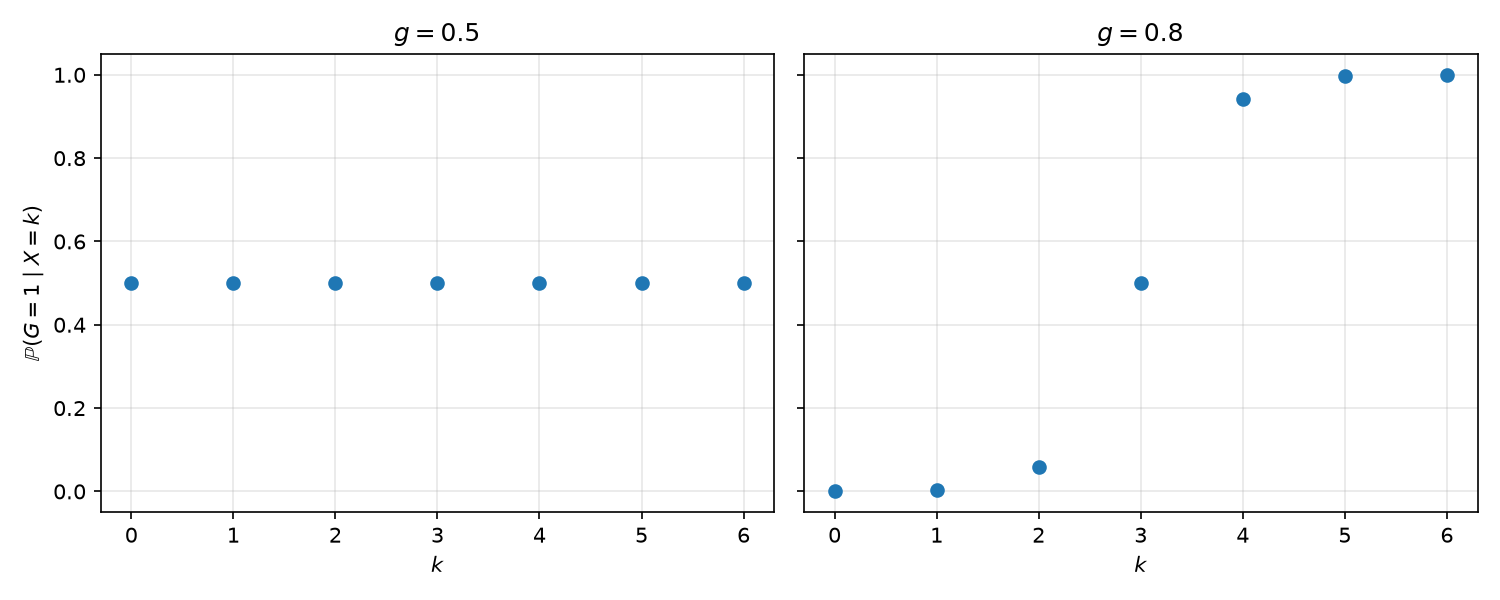
\includegraphics[width=0.75\linewidth]{math3235/posterior_scatter.png}
    \end{center}

    Shape is justified since if $g = 1/2 = b,$ then there is no way to tell the difference between the good doctor and the bad doctor from just the number of successes. Otherwise, when $g = 0.8$ and $b = 0.2,$ the higher the number of successes, the more likely it was the good doctor who achieved them. When $X = n/2,$ both doctors are equally likely.
        \end{enumerate}

\end{enumerate}
\end{document}